\def\year{2022}\relax
%File: formatting-instructions-latex-2022.tex
%release 2022.1
\documentclass[letterpaper]{article} % DO NOT CHANGE THIS
\usepackage{aaai22}  % DO NOT CHANGE THIS
\usepackage{times}  % DO NOT CHANGE THIS
\usepackage{helvet}  % DO NOT CHANGE THIS
\usepackage{courier}  % DO NOT CHANGE THIS
\usepackage[hyphens]{url}  % DO NOT CHANGE THIS
\usepackage{graphicx} % DO NOT CHANGE THIS
\urlstyle{rm} % DO NOT CHANGE THIS
\def\UrlFont{\rm}  % DO NOT CHANGE THIS
\usepackage{natbib}  % DO NOT CHANGE THIS AND DO NOT ADD ANY OPTIONS TO IT
\usepackage{caption} % DO NOT CHANGE THIS AND DO NOT ADD ANY OPTIONS TO IT
\DeclareCaptionStyle{ruled}{labelfont=normalfont,labelsep=colon,strut=off} % DO NOT CHANGE THIS
\frenchspacing  % DO NOT CHANGE THIS
\setlength{\pdfpagewidth}{8.5in}  % DO NOT CHANGE THIS
\setlength{\pdfpageheight}{11in}  % DO NOT CHANGE THIS
\usepackage{multirow}
\usepackage{graphicx}

% These are recommended to typeset algorithms but not required. See the subsubsection on algorithms. Remove them if you don't have algorithms in your paper.
\usepackage{algorithm}
\usepackage{algorithmic}
\usepackage{amsmath}
\usepackage{booktabs}
\usepackage{xcolor}
\usepackage{soul}
\newcommand*{\Scale}[2][4]{\scalebox{#1}{$#2$}}%
\newcommand*{\Resize}[2]{\resizebox{#1}{!}{$#2$}}%
\newcommand{\bl}[1]{{\textsf{\textcolor{blue}{[Bertram: #1]}}}}
\newcommand{\cam}[1]{{\textsf{\textcolor{red}{[cr:#1]}}}}

\definecolor{neonfuchsia}{rgb}{1.0, 0.25, 0.39}
\newcommand{\yiren}[1]{{\small\textcolor{neonfuchsia}{\bf [*** Yi-Ren: #1]}}}
\newcommand{\vt}[1]{{\small\textcolor{blue}{\bf [*** Vetle: #1]}}}
%
% These are are recommended to typeset listings but not required. See the subsubsection on listing. Remove this block if you don't have listings in your paper.
\usepackage{newfloat}
\usepackage{listings}
\lstset{%
	basicstyle={\footnotesize\ttfamily},% footnotesize acceptable for monospace
	numbers=left,numberstyle=\footnotesize,xleftmargin=2em,% show line numbers, remove this entire line if you don't want the numbers.
	aboveskip=0pt,belowskip=0pt,%
	showstringspaces=false,tabsize=2,breaklines=true}
\floatstyle{ruled}
\newfloat{listing}{tb}{lst}{}
\floatname{listing}{Listing}
%
%\nocopyright
%
% PDF Info Is REQUIRED.
% For /Title, write your title in Mixed Case.
% Don't use accents or commands. Retain the parentheses.
% For /Author, add all authors within the parentheses,
% separated by commas. No accents, special characters
% or commands are allowed.
% Keep the /TemplateVersion tag as is
\pdfinfo{
/Title (AAAI Press Formatting Instructions for Authors Using LaTeX -- A Guide)
/Author (AAAI Press Staff, Pater Patel Schneider, Sunil Issar, J. Scott Penberthy, George Ferguson, Hans Guesgen, Francisco Cruz, Marc Pujol-Gonzalez)
/TemplateVersion (2022.1)
}

% DISALLOWED PACKAGES
% \usepackage{authblk} -- This package is specifically forbidden
% \usepackage{balance} -- This package is specifically forbidden
% \usepackage{color (if used in text)
% \usepackage{CJK} -- This package is specifically forbidden
% \usepackage{float} -- This package is specifically forbidden
% \usepackage{flushend} -- This package is specifically forbidden
% \usepackage{fontenc} -- This package is specifically forbidden
% \usepackage{fullpage} -- This package is specifically forbidden
% \usepackage{geometry} -- This package is specifically forbidden
% \usepackage{grffile} -- This package is specifically forbidden
% \usepackage{hyperref} -- This package is specifically forbidden
% \usepackage{navigator} -- This package is specifically forbidden
% (or any other package that embeds links such as navigator or hyperref)
% \indentfirst} -- This package is specifically forbidden
% \layout} -- This package is specifically forbidden
% \multicol} -- This package is specifically forbidden
% \nameref} -- This package is specifically forbidden
% \usepackage{savetrees} -- This package is specifically forbidden
% \usepackage{setspace} -- This package is specifically forbidden
% \usepackage{stfloats} -- This package is specifically forbidden
% \usepackage{tabu} -- This package is specifically forbidden
% \usepackage{titlesec} -- This package is specifically forbidden
% \usepackage{tocbibind} -- This package is specifically forbidden
% \usepackage{ulem} -- This package is specifically forbidden
% \usepackage{wrapfig} -- This package is specifically forbidden
% DISALLOWED COMMANDS
% \nocopyright -- Your paper will not be published if you use this command
% \addtolength -- This command may not be used
% \balance -- This command may not be used
% \baselinestretch -- Your paper will not be published if you use this command
% \clearpage -- No page breaks of any kind may be used for the final version of your paper
% \columnsep -- This command may not be used
% \newpage -- No page breaks of any kind may be used for the final version of your paper
% \pagebreak -- No page breaks of any kind may be used for the final version of your paperr
% \pagestyle -- This command may not be used
% \tiny -- This is not an acceptable font size.
% \vspace{- -- No negative value may be used in proximity of a caption, figure, table, section, subsection, subsubsection, or reference
% \vskip{- -- No negative value may be used to alter spacing above or below a caption, figure, table, section, subsection, subsubsection, or reference

\setcounter{secnumdepth}{0} %May be changed to 1 or 2 if section numbers are desired.

% The file aaai22.sty is the style file for AAAI Press
% proceedings, working notes, and technical reports.
%

% Title

% Your title must be in mixed case, not sentence case.
% That means all verbs (including short verbs like be, is, using,and go),
% nouns, adverbs, adjectives should be capitalized, including both words in hyphenated terms, while
% articles, conjunctions, and prepositions are lower case unless they
% directly follow a colon or long dash
\title{\textit{KAER}: A Knowledge Augmented Pre-Trained Language Model for Entity Resolution}
% \author{
%     Anonymous Authors
% }

%Example, Single Author, ->> remove \iffalse,\fi and place them surrounding AAAI title to use it
\iffalse
\title{My Publication Title --- Single Author}
\author {
    Author Name
}
\affiliations{
    Affiliation\\
    Affiliation Line 2\\
    name@example.com
}
\fi

\iffalse
%Example, Multiple Authors, ->> remove \iffalse,\fi and place them surrounding AAAI title to use it
\title{My Publication Title --- Multiple Authors}
\author {
    % Authors
    First Author Name,\textsuperscript{\rm 1}
    Second Author Name, \textsuperscript{\rm 2}
    Third Author Name \textsuperscript{\rm 1}
}
\affiliations {
    % Affiliations
    \textsuperscript{\rm 1} Affiliation 1\\
    \textsuperscript{\rm 2} Affiliation 2\\
    firstAuthor@affiliation1.com, secondAuthor@affilation2.com, thirdAuthor@affiliation1.com
}
\fi


% REMOVE THIS: bibentry
% This is only needed to show inline citations in the guidelines document. You should not need it and can safely delete it.
\usepackage{bibentry}
% END REMOVE bibentry

\begin{document}

\maketitle

\begin{abstract}

Entity resolution is an important and well-studied task for decades, while it is challenging and expensive to apply the traditional way of matching entities with long sequences of textual data and a large dataset, nor hard to compare the data without recognizing the resourceful semantic data information without domain knowledge. 

In this study, we propose a novel framework for incorporating external knowledge into pre-trained language model for entity resolution. We discussed the results of utilizing different knowledge augmentation and prompting methods to improve entity resolution performance, and we assume a deeper language understanding of the entity resolution problems. 

% name not define 
According to our experiment results, our model achieves better results than Ditto, the existing state-of-the-art entity resolution method. 


\end{abstract}


\section{Introduction}
% PLMs rarely used in data cleaning, in particular, entity resolution tasks
%  challenge 1: missing domain knowledge to help prepare data;
%  challenge 2: missing semantic data types/ a better language understanding of the textual data
%  challenge 3: "too much knowledge incorporation may divert the sentence
% from its correct meaning, which is called knowledge
% noise (KN) issue." \cite{liu_k-bert_2020}
Recent studies using \emph{transformer-based Pre-trained Language Models} (PLMs) have shown their strong ability to perform various types of NLP tasks \cite{min_recent_2021}. However, few studies have discussed the application of PLMs in the domain of data cleaning~\cite{li_deep_2020,narayan_can_2022,vos2022towards}.  
Entity resolution is a common data cleaning task that aims to identify the entries referring to the same real-world entities within or across databases~\cite{christen_data_2012}. 
% \bl{Entity resolution is a common data cleaning task ...}


% Entity resolution, also known as entity matching, record linkage, or data deduplication, is a classical problem in data integration~\cite{zhao_auto-em_2019}. 
% The typical process of entity resolution contains data preparation, data indexing or blocking, and data matching. %  challenge 1: missing domain knowledge to help prepare data;

% Prior work has shown that data 
% Prior work has shown that performing data cleaning before applying ML-based models for entity resolution can improve task performance,  e.g., tokenization or stemming, for threshold-based classifiers \cite{koumarelas_data_2020}.
% \bl{This sentence needs to be re-written for clarity.}.  
% However, it still remains under-studied how data preparators can be applied to datasets from different domains or different types. \bl{it is still an open problem how data preparatory can be applied ... and different data types} For instance,



% \bl{Most ...... the same schema ...., however, in many situations, data from different sources are heterogeneous and use different schema.(heterogeneous schema}

Most existing techniques on entity resolution assume the same schema for records from different sources \cite{elmagarmid_duplicate_2007}. However, in many situations, raw records are obtained from heterogeneous sources and use different schema \cite{enriquez_entity_2017, arabnia_when_2021}. In addition, source data often cover varied domains (e.g., publications, online products, musicians) and in different formats (e.g., numerical, textual, geolocations). 
% , which adds more difficulties for entity resolution tasks 
%Christian (2012) mentioned that schema standardization of records is an essential data preparation for entity resolution task~\cite{christen_data_2012}. 
All of these increase the difficulty for practitioners to perform entity resolution tasks without prior knowledge of the domain-specific information about the data.
% Hulsebos et al \cite{hulsebos_sherlock_2019} introduced Sherlock, a multi-input deep neural network for detecting semantic data types, in which they match 78 semantic types from DBpedia to column headers.  Similarly, Doduo \cite{suhara_annotating_2022}, a multi-task learning framework that is based on
% \emph{pre-trained language models} (PLMs) can predict column types and column relations. 
Thus, we hypothesize that enhancing the external knowledge at the schema and entity level can improve entity resolution tasks.  

With transformer-based PLMs, recent studies draw increasing attention to entity resolution problems~\cite{li_deep_2020, trabelsi_dame_2022}. However, current studies show that the performance might not be ideal when simply inputting the serialized entity pairs into PLMs for classification. Ditto \cite{li_deep_2020} injects domain information: pre-defined entity types (i.e., PRODUCT and NUM), and standardizes the numerical formats to improve the performance before feeding the serialized entity pairs into PLMs.

We push this idea further by injecting more external knowledge at the schema and entity level. Knowledge injection at the schema level aims to infer the fine-grained semantic types (e.g., ALBUM, ARTIST, PUBLISHER) for each column based on data values. 
For the entity level, entity mentions are identified from WikiData and annotated in the initial text with semantic type information of the linked entities. In addition, different formats used to inject external knowledge into the initial entity pairs may vary the performance of PLMs. Thus, three prompting methods are further explored in this study: space, slash, and additional position encoding of PLMs.
% soft position encoding with the visible matrix. 

% Contributions:?
To summarize, starting from state-of-the-art method Ditto \cite{li_deep_2020}, we propose a framework for  \textbf{K}nowledge \textbf{A}ugmented \textbf{E}ntity \textbf{R}esolution (KAER):
\begin{itemize}
    \item using \textbf{C}olumn \textbf{S}emantic \textbf{T}ype (CST) inference and \textbf{E}ntity \textbf{L}inking (EL) in order to inject domain-specific information as additional signals to pre-trained language models. 
    \item leveraging three prompting methods to better augment the acquired knowledge to PLMs.
    \item analyzing the effectiveness of different knowledge injection and prompting methods on entity resolution tasks from different domains and data types.
\end{itemize}
%\vspace{-0.3cm}

% \section{Research Problems}
% In this project, we target the following research questions:
% \begin{itemize}
%     \item (RQ$_1$) How to incorporate domain knowledge into input data when using PLMs for data cleaning?
    
%     \item (RQ$_2$) To what extent does the incorporation of domain knowledge benefit downstream data cleaning tasks, such as entity resolution? 
% \end{itemize}


\section{Related Work}
\begin{figure*}[!ht]
    \centering
    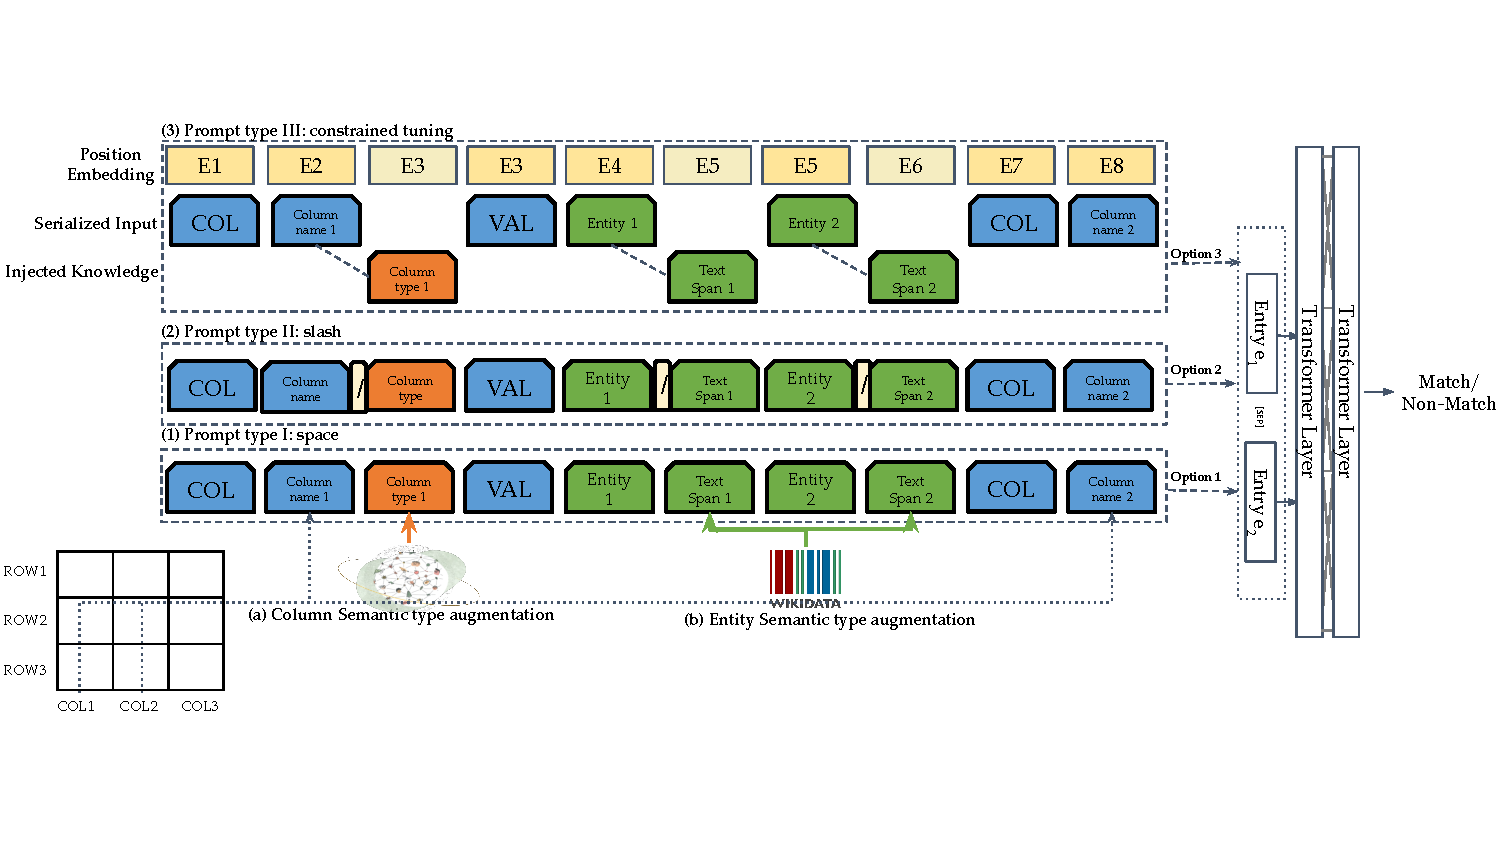
\includegraphics[width=\linewidth]{plots/DCER_short.pdf}
    \caption{The framework of KAER.}
    \vspace{-0.5cm}
    \label{fig:framework}
\end{figure*}

% \subsection{Data Preparation: a Preceding Stage of Entity Resolution}

% Data quality impacts the cost and performance of entity resolution systems significantly. Even for an error-free system with perfectly clean data, data from multiple sources are often not saved in a consistent way or carefully controlled for quality \cite{elmagarmid_duplicate_2007}. Usually, the data preparation stage includes parsing, data transformation, and standardization steps, and the goal is to improve the quality of the in-flow data and make the data comparable, and more usable \cite{elmagarmid_duplicate_2007}. 

% Even though adjusting and selecting data preparators to prepare data before doing the entity resolution is not the focus of this paper, we will still apply some general data transformations to deal with specific data types. Data transformations are used to convert the data into the correct type or format that conforms to their domains \cite{elmagarmid_duplicate_2007}. Enhancing data quality by preprocessing data also contributes to the result of Sherlock \cite{hulsebos_sherlock_2019}, which can detect the semantic data types. Here we mainly use general transformations to help normalize the atomic types of data, such as \textit{string}, \textit{integer}, \textit{Boolean}. For instance, the \textit{float} type of data values for $Year$ is meaningless. So a simple conversion of the data from \textit{float} to \textit{integer} is required. Meanwhile, encoding issues also appear across the data values that need to be addressed at this stage. For numerical data, range checking could be used to ensure that data is in the appropriate range \cite{elmagarmid_duplicate_2007}. Preprocessing composite data values will be more complicated that requires a few steps, i.e., we usually first split the data values and then prepare data values separately, and finally merge the cleaned data values.

% \subsection{Schema Matching: The Context of Entity Resolution}
% % Assigned to Lan Li
% Entity resolution is to identify and match records that refer to the same real-world entity. In many situations, raw records are stored from heterogeneous sources, while most existing techniques on entity resolution predefine the same schema for records from different sources \cite{elmagarmid_duplicate_2007}. Moreover, records from different sources might follow different structures at the attribute level, which adds more difficulties for entity resolution tasks \cite{enriquez_entity_2017, arabnia_when_2021}. Therefore, schema matching is required to discuss before we talk about entity resolution tasks. In particular, we consider the schema matching task as the context of processing entity resolution for schema matching guides which two records should be paired at the column level before processing the entity resolution at the row level. \cite{lin_efficient_2020} perform schema matching by creating a \textit{full schema} in which they compare and merge records from different sources into \textit{super record} before the entity resolution. In this way, they avoid information loss during the schema-matching process.

% The main operation in manipulating schema information is \textit{Match}, which inputs two schemas and produces a mapping between two elements of the two schemas that relate semantically to each other \cite{rahm_survey_2001}. \cite{rahm_survey_2001} select the matching algorithms (a.k.a matchers) based on the application domain and schema types, and use data types to constrain the search space of correspondences. 

\subsection{Pretrained Model for Entity Resolution}
% Assigned to Lan Li

% \cite{zhao_auto-em_2019} propose a transfer-learning approach to entity matching (EM), leveraging pre-trained entity matching models that are based on large-scale, production knowledge bases (KB). Auto-EM enables entity type detection and entity matching at the attribute level by learning a large amount of data from KBs. In this way, they achieve a high EM quality with little labeled training data. \cite{wu_zeroer_2020} introduce ZeroER that requires \textit{Zero} labeled examples for entity resolution task. They leverage a powerful generative model based on Gaussian Mixture Models for learning the match and mismatch distributions. 

% Unlike Recurrent Neural Network (RNN) used in \cite{zhao_auto-em_2019, mudgal_deep_2018}, 
A few recent works apply transformer-based PLMs to entity resolution tasks. \citet{paganelli_analyzing_2022} discover that simply fine-tuning BERT can benefit to matching/non-matching classification tasks and BERT can recognize the input sequence as a pair of records. \citet{li_improving_2021} leverage siamese network structure to PLMs in order to improve the efficiency of PLMs during the blocking phase. 
Ditto by \cite{li_deep_2020} is now the state-of-the-art entity matching system based on pre-trained Transformer-based language models. In addition, Ditto provides a deeper language understanding for entity resolution by injecting domain knowledge, summarizing the key information, and augmenting with more difficult examples for training data. 
% Ditto injects dataset type and numeric data type as the domain knowledge. Inspired by ditto, we aim to corporate column type semantic and e
 
% Auto-EM introduce the framework to pretrain an RNN-based attribute type classifier on large knowledge base .
\vspace{-0.5em}
\subsection{Knowledge Augmentation}
Recent works show that injecting external knowledge to PLMs can benefit Natural Language Reprocessing (NLP) downstream tasks~\cite{zhang_ernie_2019,peters_knowledge_2019,liu_k-bert_2020,wang_k-adapter_2021, wang_kepler_2021}. 
There are existing studies about methods that can be used to inject external domain knowledge into PLMs: 

% \subsection{Semantic data types recognition at column-level}

\subsubsection{Semantic column type detection}
Sherlock \cite{hulsebos_sherlock_2019} is a novel system that uses a deep learning approach to detect semantic data types at the column level. Sherlock predicts the conceptual domain of a column when there is no schema or the existing schema cannot provide a fine-grained description of the data. Doduo~\cite{suhara_annotating_2022} is another recent method for annotating  columns with semantic types and for adding semantic relations between columns. Both Sherlock and Doduo methods can be used to inject domain-specific knowledge for columns with existing names or missing names.

\subsubsection{Entity linking}
Entity linking \cite{li_deep_2020} refers to the task of linking entity mentions appearing in natural language text with their corresponding entities in an external knowledge base, e.g., Wikidata. 
Existing study has explored using PLMs to perform entity linking tasks, and achieved promising results. 
\citet{zhang_ernie_2019} introduced the model ERNIE by jointly pre-training BERT with a masked language modeling objective. The knowledge augmented BERT model is found to outperform existing methods in multiple knowledge-driven tasks. 
Later work by \citet{peters_knowledge_2019} futher improved the ERNIE model by introducing a trainable entity linker module and alignment between entity embedding and BERT embedding. 
Recent work by \citet{ayoola_refined_2022} introduced an entity linking method by using fine-tuning a pre-trained language model over Wikipedia data. The model has shown strong ability in zero-shot domain adaptation, which is used as a baseline method for entity linking in our study. 

\subsubsection{Knowledge prompting} %\liri{Liri}
The method of conditioning the language model, a.k.a, "prompting," is a hot topic in Nature Language Processing \cite{kojima_large_2022}. They \cite{kojima_large_2022} propose Zero-shot-CoT, a single zero-shot prompt that evokes a chain of thought from large language models, highlighting that the performance of the language model has been affected by different templates of the prompt.
Furthermore, the method to inject the identified external knowledge into PLMs matters. \citet{liu_k-bert_2020} propose the model K-BERT adding soft-position encoding and visible matrix to the augmented input sequence to avoid exposing too much knowledge to the original input and corresponding models. 
%Another direction of knowledge incorporation is to align the knowledge embedding and PLMs output into same embedding space. The work from Wang et al. \cite{wang_kepler_2021} introduced a joint pre-training method based on roBERTa to map knowledge base entity and natural language entity description into the sample space. The knowledge embedding produced by KEPLER can be utilized as an additional input information source in our entity resolution task. The effectiveness of these methods in incorporating knowledge into entity resolution tasks can be further explored.




\section{Methodology}
\begin{table*}[!ht]
\centering
\resizebox{\linewidth}{!}{
\begin{tabular}{lccccccc}
\hline
\multicolumn{1}{l|}{}                  & \multicolumn{2}{c|}{\textbf{Dirty}} & \multicolumn{4}{c|}{\textbf{Structured}}                      & \textbf{Textual} \\ \hline
\multicolumn{1}{c|}{\textbf{Injection}} &
  \textbf{\begin{tabular}[c]{@{}c@{}}DBLP\\ -\\ GoogleScholar\end{tabular}} &
  \multicolumn{1}{c|}{\textbf{\begin{tabular}[c]{@{}c@{}}iTunes\\ -\\ Amazon\end{tabular}}} &
  \textbf{\begin{tabular}[c]{@{}c@{}}iTunes\\ -\\ Amazon\end{tabular}} &
  \textbf{\begin{tabular}[c]{@{}c@{}}Amazon\\ -\\ Google\end{tabular}} &
  \textbf{\begin{tabular}[c]{@{}c@{}}DBLP\\ -\\ ACM\end{tabular}} &
  \multicolumn{1}{c|}{\textbf{\begin{tabular}[c]{@{}c@{}}DBLP\\ -\\ GoogleScholar\end{tabular}}} &
  \textbf{\begin{tabular}[c]{@{}c@{}}Abt\\ -\\ Buy\end{tabular}} \\ \hline
\textbf{Ditto}                         & 95.8             & 66.7             & 85.2          & 73.2          & 98.8          & 95.9          & 88.4             \\
\textbf{Ditto + Sherlock}              & 95.8             & \textbf{90.2}    & \textbf{92.6} & 67.3          & 98.8          & 94.3          & 89.2             \\
\textbf{Ditto + Sherlock + /}          & 95.7             & 90.0             & 88.9          & 70.0          & 98.7          & 95.5          & 91.7             \\
\textbf{Ditto + Sherlock + KBert}      & 95.3             & 66.7             & 66.7          & 77.9          & 97.5          & 95.7          & 77.2             \\
\textbf{Ditto + Doduo}                 & 94.8             & 88.5             & 66.7          & 72.5          & 98.8          & 95.6          & 88.6             \\
\textbf{Ditto + Doduo + /}             & 95.4             & 80.0             & 53.6          & \textbf{76.6} & 98.8          & 95.7          & 88.9             \\
\textbf{Ditto + Doduo + KBert}         & 95.5             & 72.0             & 72.7          & 75.4          & 96.9          & 95.6          & 69.4             \\
\textbf{Ditto + EL}                    & 95.6             & 87.3             & 72.4          & 73.5          & 98.5          & 95.5          & 89.1             \\
\textbf{Ditto + EL + /}                & 95.5             & 80.8             & 84.6          & 73.1          & 98.4          & \textbf{96.2} & 88.2             \\
\textbf{Ditto + EL + KBert}            & 95.2             & 80.9             & 69.7          & 76.2          & 97.1          & 95.3          & 74.8             \\
\textbf{Ditto + Sherlock + EL}         & 95.7             & 69.7             & 73.5          & 71.7          & 98.4          & \textbf{96.2} & 89.7             \\
\textbf{Ditto + Sherlock + EL + /}     & \textbf{96.0}    & 75.4             & 61.5          & 75.5          & 98.3          & 95.2          & 89.8             \\
\textbf{Ditto + Sherlock + EL + KBert} & 94.8             & 66.7             & 70.0          & 73.5          & 96.5          & 94.7          & 66.8             \\
\textbf{Ditto + Doduo + EL}            & 95.2             & 62.5             & 66.7          & 74.4          & \textbf{99.0} & 95.8          & \textbf{92.1}    \\
\textbf{Ditto + Doduo + EL + /}        & 95.3             & 62.5             & 54.5          & 75.5          & 98.8          & 95.4          & 89.0             \\
\textbf{Ditto + Doduo + EL + KBert}    & 94.1             & 69.2             & 71.7          & 76.2          & 95.8          & 94.9          & 56.7             \\ \hline
\end{tabular}
}
\caption{Results using different knowledge injection methods.}
\label{tab:injection_results}
\end{table*}



\subsection{Notation of Entity Resolution Task}
We now describe the formulation of the entity resolution task we will focus on in this paper. The input of the entity resolution task consists of a set $M \subseteq D_1 \times D_2$ of data entries $e \in M$, where $D_1$ and $D_2$ are two sets of data entry collections that contain duplicated entries. 
For each data entry, $e \in {(attr_i, val_i)}_{1 \leq i \leq N}$ where $N$ is the size of the set $M$, and $(e_1, e_2) \in M$. The task discussed in this paper focuses on: for each data entry pair $(e_1, e_2) \in M$, determine whether this pair is a pair of duplicated data entries.
% \yiren{TODO}

\subsection{Overview}


\subsubsection{Pre-trained Language Model for Entity Resolution}
Following the work by Li et al. \cite{li_deep_2020}, we use roBERTa-based as the backbone model of our entity resolution method. For each data entry pair $(e_1, e_2)$, we serialize the text context of column names and values of $e_1$ and $e_2$, and concatenate them as the input for language model. We then use the [CLS] token position to classify whether $e_1$ and $e_2$ refer to the same entity. 
The loss for optimizing the classification objective is:

\begin{equation}
    \ell = - log\ p(y | e_1, e_2)
\end{equation}

where y denotes whether $e_1$ and $e_2$ refer to the same entity. 


% \subsubsection{Knowledge Augmentation}

\subsubsection{Column Type Prediction}
Column type prediction aims to predict the semantic type of each column by considering the context of inter- and intra-columns. We leverage two methods for column type prediction: Sherlock \cite{hulsebos_sherlock_2019} and Doduo \cite{suhara_annotating_2022}.

\textbf{Sherlock} is a multi-input deep neural network and is trained on 686,765 data columns retrieved from the VizNet corpus by matching 78 semantic data types from DBpedia to column headers \cite{hulsebos_sherlock_2019}. There are four categories of features fed into this neural network, including global statistics, aggregated character distributions, pre-trained word embeddings, and self-trained paragraph vectors. Overall, they train subnetworks for aggregated character distributions, pre-trained word embeddings, and paragraph vectors. And then they concatenate the weights of the three output layers with global statistics features to form the input of Sherlock. 

\textbf{Doduo} is a multi-task learning framework based on pre-trained language models (LMs) \cite{suhara_annotating_2022}. Doduo serializes the entire table into a sequence of tokens to make it fit for Transformer-based architecture. Considering a table T consists of a set of attributes, i.e., $T= (c_1, c_2,... c_n)$, and we denote by  $val(T.c_i)$ the list of data values stored at the column $c_i$. In this way, for each value v, it can be of string type and split into a sequence of input tokens to pre-trained LMs. The serialization strategy of Doduo is simply concatenating column values to make a sequence of tokens and feed that sequence as input to the model \cite{suhara_annotating_2022}. 

\begin{equation}
    serialize_{single}(C) ::= [CLS]\ v_1\ ...\ v_m\ [SEP],
\end{equation}

[CLS] and [SEP] are special tokens to mark the beginning and end of a sequence. 


\subsubsection{Entity linking}
The task of entity link aims to identify all entity mentions from a given knowledge base (KB) within the target text sequence. More specifically, we attempt to identify the text span of each entity mention $m \in M$, and map each mention to the entity set from an external KB $\mathcal{M}: M \rightarrow E$. 
We then use additional knowledge from the KB to augment the input text records.
In this study, we use WikiData as the external KB since it covers a wide range of domains and is suitable for entity resolution over different datasets. For the entity linking method, we use the state-of-the-art method proposed by Ayoola et al. \cite{ayoola_refined_2022}, which uses a RoBERTa model jointly pre-trained over entity typing and entity description modeling objectives. We extract the coarse entity type as the additional knowledge we inject into the model input.

% \subsubsection{Prompting for Knowledge Injection}

\subsubsection{Template-based prompting}
After acquiring domain knowledge, we experiment using text-based template to combine the knowledge with the initial text input. We concatenate the original entity mention/column name with the injected knowledge text with a "/" token. The "/" is the same token as "/" in the text. 
Additionally, we also experiment with simply using space to connect the original entity mention/column name and injected knowledge. 


% \begin{equation}
%     s(e_1, e_2) ::= [COL] attr_i [VAL] val_i [SEP] [COL] attr_j [val] val_j
% \end{equation}

\subsubsection{KBert}





\section{Experiments}
% TODO: dataset statistic table
\subsection{Dataset}

KAER is evaluated on the Magellan datasets \cite{magellandata} across various domains. 
%The data collection contains datasets designed for entity matching tasks . 
The overview of the datasets used in this study is shown in Table~\ref{tab:dataset_overview}. 
The Magellan datasets contain three types of datasets: dirty dataset, structured dataset, and textual dataset.
In particular, the dirty version of datasets is generated from the clean version by randomly removing values of attributes and appending the initial values to another randomly selected attribute~\cite{li_deep_2020}.

\begin{table}[h]
\centering
\resizebox{\columnwidth}{!}{%
\begin{tabular}{lclccc}
\hline
\textbf{Data Type} & \textbf{Dataset} & \textbf{Domain} & \textbf{Size} & \textbf{\# Positive} & \textbf{\# Attr.} \\ \hline
Structured             & Amazon-Google      & software & 11,460 & 1,167 & 3 \\
                       & iTunes-Amazon      & music    & 539    & 132   & 8 \\
                       & DBLP-ACM           & citation & 12,363 & 2,220 & 4 \\
                       & DBLP-GoogleScholar & citation & 28,707 & 5,347 & 4 \\ \hline
\multirow{3}{*}{Dirty} & iTunes-Amazon      & music    & 539    & 132   & 8 \\
                       & DBLP-ACM           & citation & 12,363 & 2,220 & 4 \\
                       & DBLP-GoogleScholar & citation & 28,707 & 5,347 & 4 \\ \hline
Textual                & Abt-Buy            & product  & 9,575  & 1,028 & 3 \\ \hline
\end{tabular}
}
\caption{Dataset Summary}
\label{tab:dataset_overview}
\vspace{-0.5cm}
\end{table}

% \subsection{Implementation Details}
% We use RoBERTa-base as the backbone model. 






\subsection{Results}
The experimental results are presented in Table \ref{tab:injection_results}.


\textit{Knowledge injection performs better on smaller datasets.}
According to the experimental results, incorporating external knowledge can improve the performance on entity resolution tasks. In particular, the proposed knowledge augmentation methods outperform the two baseline models in a data-scarce context.
% This improvement is found to be more significant on datasets with a smaller amount of training data. 
% The results show that our proposed knowledge augmentation methods can improve the model performance over the state-of-the-art Ditto model, especially in a data-scarce context. 
% the F1 score of most knowledge injection methods and prompting methods are higher than the F1 score of baseline model Ditto 
For example, \textbf{KAER (RoBERTa + CST)} outperforms both baseline models Roberta and Ditto by 23.5\% and 13.1\% $\uparrow$ on dataset Dirty/iTunes-Amazon and 7.4\% and 38.8\% $\uparrow$ on dataset Structured/iTunes-Amazon. The two baseline models perform worse on smaller datasets because the language model might not be able to learn enough information to distinguish between different entities, given fewer training instances correctly. 
 % \textit{Prompting with "/" performs better than space and K-BERT style injection.}
Through prompting, the model is provided with additional knowledge to augment the learning process. The experimental results revealed that using slash ``/'' to prompt the model with additional knowledge performs better than using space and \textbf{A}dditional \textbf{P}osition \textbf{E}ncoding (APE) prompting in most scenarios. For example, \textbf{KAER (RoBERTa+CST+EL+/)} performs better than the other two prompting methods 
%space and APE \textbf{KAER (RoBERTa+CST+EL)} and \textbf{KAER(RoBERTa+CST+EL+APE)} 
on dataset Dirty/DBLP-GoogleScholar. Moreover, prompting with APE achieved better performance in datasets with smaller text lengths. For example, \textbf{KAER (RoBERTa+CST+APE} reaches the best F1 score (77.9\%) on dataset Structured/Amazon-Google, which contains the smallest text lengths.  

\textit{Knowledge injection does not perform well datasets from certain domains.}
The datasets used in our experiments span several different domains. Using our proposed knowledge augmentation methods (e.g., entity linking), records from certain domains, such as music and online product, benefit from more accurate retrieved knowledge. For example, \textbf{KAER(RoBERTa+CST)} achieves the best F1-score on the musical dataset iTunes-Amazon, as analyzed above, it outperforms both baseline models significantly. \textbf{KAER(RoBERTa+CST+/)} achieves the best F1-score, i.e., 91.7\%, on the textual dataset Abt-Buy from the online product domain. One potential reason for this notable improvement is that the entities mentioned in the datasets from these domains are more general.
However, publication datasets from domains like citation require more domain-specific or even expert knowledge rather than general commonsense. Our knowledge injection methods are primarily designed for retrieving general knowledge. Thus, for datasets, like Structured/DBLP-ACM, \textbf{KAER(RoBERTa+CST)} performs as well as the baseline model, achieving the best F1-score 98.8\%, \textbf{RoBERTa}, but all the other KAER models perform worse. For future improvement, additional external expert knowledge from the citation domain should be incorporated for knowledge injection. 
% \vt{The knowledge injection does not help in highly domain-specific dataset. The knowledge we are injecting is not the correct knowledge in terms of domain.}

\textit{Knowledge augmentation is affected by data quality.}
%We notice that 
KAER, with knowledge augmentation methods, outperforms the baseline models on dirty datasets. However, F1 scores on the dirty version of the dataset DBLP-GoogleScholar are lower than the results on the structured version (cleaner version). One reason might be that the misleading predictions based on the dirty input by CST result in semantic noise and propagate to the PLMs.
On the other hand, according to the results, knowledge augmentation can advance the robustness of the model on low-quality data. For instance, \textbf{KAER+CST} and \textbf{KAER+CST+EL+/} outperform both baseline models with the dirty datasets.
% which verifies the importance and necessity of knowledge augmentation for better language understanding on entity resolution tasks.


% The prediction performance of our model heavily relies on the quality of the input dataset, in particular, the semantic column types based on the characteristics of the input data.  
 



% For instance, the dirty version of iTunes-Amazon dataset is generated from the clean version by randomly emptying attributes and appending their values to another randomly selected
% attribute \cite{li_deep_2020}.
% \textit{Cascading error from knowledge injector leads to lower performance.} 
% xxx


\section{Conclusion}
% Results/Future work: different domains
% Issues/Motivations: web content (noisy data: value + schema)
% Solutions: Augmented with Knowledge prompts (extra domain knowledge + prompting methods)

In this study, we introduced a framework for addressing entity resolution problems by incorporating external knowledge using prompting techniques. We evaluated our method over a set of datasets from varied domains, and achieved higher performance than state-of-the-art entity resolution method. 
Future study can improve upon our method by introducing more domain-specific knowledge. 


\section{Acknowledgement}
The experiments are conducted on the NCSA Delta supercomputing system, supported by the National Science Foundation under Grant No. OAC-2005572.  

\bibliography{Reference}

\section{APPENDIX}
\paragraph{A. Hyperparameter Settings.} 
Baseline and KAER models share the same hyperparameter setting, in which the batch size equals 64, the max length equals 512, the learning rate is 3e-5, and the number of training epochs is 20. 
%Other parameters keep unchanged with the default setting from Ditto. 
%-lr", type=float, default=3e-5)
%    parser.add_argument("--n_epochs", type=int, default=20)

\paragraph{B. Baseline models.} 
\begin{table}[!b]
\centering
\begin{tabular}{|l|l|}
\hline
Dataset                  & Injection       \\ \hline
dirty/DBLP-Google        & Ditto + General \\ \hline
dirty/iTunes-Amazon      & Ditto + Product \\ \hline
structured/iTunes-Amazon & Ditto + Product \\ \hline
structured/Amazon-Google & Ditto + Product \\ \hline
structured/DBLP-ACM      & Ditto + General \\ \hline
structured/DBLP-Google   & Ditto + General \\ \hline
textual/Abt-Buy          & Ditto + Product \\ \hline
\end{tabular}
\caption{Datasets and Corresponding Ditto default knowledge injection methods}
\label{tab:dittoinject}
\end{table}
This paper includes two baseline models, i.e., RoBERTa without any knowledge injection and Ditto with its default knowledge injection methods. 

In detail, Table~\ref{tab:dittoinject} shows the datasets and corresponding injection methods utilized by Ditto. "+ General" indicates that Ditto injects seven entity types into the corresponding dataset. The seven types include 'PERSON', 'ORG', 'LOC', 'PRODUCT', 'DATE', 'QUANTITY', and 'TIME'. "+ Product" indicates that Ditto annotates as 'PORODUCT', any entity mentions in the following types, i.e., 'NORP', 'GPE', 'LOC', 'PERSON', and 'PRODUCT'.

\paragraph{C. Two-sided Paired T-test.}
The two-sided paired T-test is implemented to test whether the predictions of different models are significantly different. We first compare whether the predicted label is equal to the ground-truth label. The value is 1 if the prediction is equal to the ground truth and 0 otherwise. And then, the paired T-test is conducted. 
% \begin{table*}[!h]
% \centering
% \resizebox{\linewidth}{!}{
% \begin{tabular}{l|ll|llll|l}
% \hline
% \multicolumn{1}{l|}{}                  & \multicolumn{2}{c|}{\textbf{Dirty}} & \multicolumn{4}{c|}{\textbf{Structured}}                      & \textbf{Textual} \\ \hline
% \multicolumn{1}{l|}{\textbf{Models}} &
%   \textbf{\begin{tabular}[l]{@{}l@{}}DBLP\\ -\\ GoogleScholar\end{tabular}} &
%   \multicolumn{1}{c|}{\textbf{\begin{tabular}[l]{@{}l@{}}iTunes\\ -\\ Amazon\end{tabular}}} &
%   \textbf{\begin{tabular}[l]{@{}l@{}}iTunes\\ -\\ Amazon\end{tabular}} &
%   \textbf{\begin{tabular}[l]{@{}l@{}}Amazon\\ -\\ Google\end{tabular}} &
%   \textbf{\begin{tabular}[l]{@{}l@{}}DBLP\\ -\\ ACM\end{tabular}} &
%   \multicolumn{1}{l|}{\textbf{\begin{tabular}[l]{@{}l@{}}DBLP\\ -\\ GoogleScholar\end{tabular}}} &
%   \textbf{\begin{tabular}[c]{@{}l@{}}Abt\\ -\\ Buy\end{tabular}} \\ \hline
% RoBERTa                          & 95.81                             & 72.73                       & 61.76                       & 73.12                       & 98.77                   & 95.32                             & 88.41                                \\
% Ditto                            & 95.54                             & 60.38                       & 47.06                       & 74.44                       & 98.55                   & 95.85                             & 88.89                                \\ \hline
% KAER ( Roberta + CST )           & 95.47                             & 62.96                       & 80.70**++                   & 68.70                       & 98.77                   & 95.05                             & 92.27**++                            \\
% KAER ( Roberta + CST + / )       & 95.74                             & 54.90*                      & \textbf{89.66**++}          & 74.85                       & \textbf{98.99}          & 95.14                             & \textbf{92.61**++}                   \\
% KAER ( Roberta + CST + PCT)      & 95.20                             & 72.00                       & 57.14                       & \textbf{76.25}              & 98.09*                  & 95.62                             & 78.24**++                            \\
% KAER ( Roberta + EL )            & 95.12                             & 50.00*                      & 61.54                       & 73.77                       & 98.54                   & 95.72                             & 89.11                                \\
% KAER ( Roberta + EL + / )        & 95.75                             & \textbf{81.82}              & 86.21**++                   & 74.02                       & 98.43                   & \textbf{96.11*}                   & 88.19                                \\
% KAER ( Roberta + EL + PCT)       & 94.80**+                          & 77.78+                      & 67.69                       & 75.63                       & 97.04**+                & 95.29                             & 73.80**++                            \\
% KAER ( Roberta + CST + EL )      & \textbf{95.87}                    & 47.06*                      & 59.26                       & 72.28                       & 98.43                   & 95.65                             & 89.66                                \\
% KAER ( Roberta + CST + EL + / )  & 95.63                             & 63.33*                      & 57.14+                      & 75.15                       & 98.34                   & 95.67                             & 89.81                                \\
% KAER ( Roberta + CST + EL + PCT) & 94.24**++                         & 71.11+                      & 61.29                       & 71.37*                      & 96.26**++               & 94.93+                            & 67.20**++                            \\ \hline
% \end{tabular}
% }
% \vspace{-0.2cm}
% \caption{Experimental results using different knowledge injection methods, measured by F1 score. 
% % 99\% and 95\% confidence level of hypothesis test (paired t-test).
% The two baseline models: RoBERTa (without domain knowledge injection); and Ditto (RoBERTa and Ditto's general domain knowledge injection methods). 
% % representing the baseline model, Ditto without knowledge injection, 
% Other models represent KAER with various knowledge injection and prompting methods combined with RoBERTa. ``+CST'' indicates \textbf{C}olumn \textbf{S}emantic \textbf{T}ype injection.``+EL'' indicates knowledge injection with \textbf{E}ntity \textbf{L}inking. ``+/'' represents prompting with a slash. ``+PCT'' represents \textbf{P}rompting with \textbf{C}onstrained \textbf{T}uning, i.e., soft positions and visible matrix. The paired t-test is processed between KAER injections and two baseline models, i.e., RoBERTa(*) and Ditto(+). \textbf{**} and \textbf{++} represent 99\% confidence level, and \textbf{*} and \textbf{+} represent 95\% confidence level.}%significance level ($\alpha=0.05$).} 
% \label{tab:injection_results}
% \end{table*}

\end{document}
